\chapter{Кинетическая энергия материальной точки и системы. Теорема Кенига.
Кинетическая энергия твердого тела в поступательном, вращательном и плоском
движениях.}

\section{Кинетическая энергия материальной точки и системы}

\emph{Кинетическая энергией материальной точки называется 
скалярная величина \( mv^2/2 \), равная половине произведения 
массы точки на квадрат её скорости.}
\[ T = \frac{mv^2}{2} \]

\emph{Кинетической энергией системы называется скалярная величина 
\( T \), равная сумме кинетических энергий всех точек системы:}
\[ T = \sum T_k = \sum\frac{m_k v^2_k}{2} \]

\section{Теорема Кенига}
Кинетическая энергия системы есть энергия движения центра масс плюс энергия 
движения относительно центра масс:
\[ T = T_0 + T_r \]
где \( T \) -- полная кинетическая энергия, \( T_0 \) -- энергия движения 
центра масс, \( T_r \) -- относительная кинетическая энергия.

Полная кинетическая энергия тела или системы тел в сложном движении равна 
сумме энергий системы в поступательном движении и энергия системы во 
вращательном относительно центра масс.

\section{Кинетическая энергия твердого тела в поступательном, вращательном 
и плоском движениях}

\begin{figure}[h!]
    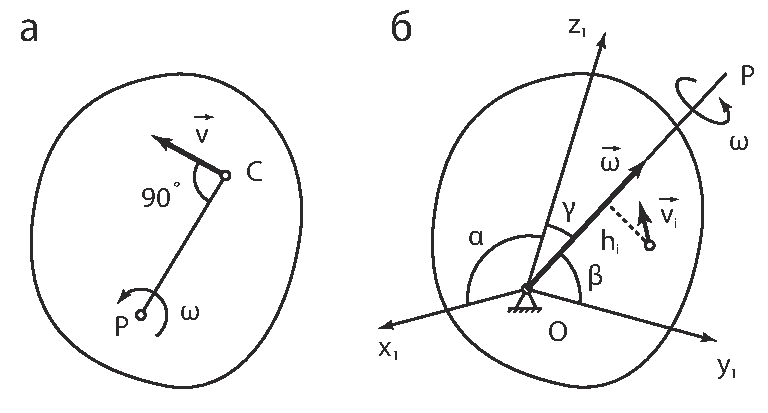
\includegraphics[width=.47\textwidth]{54_01}
    \parbox{.47\textwidth}{\caption{} \label{pic54_01}}
\end{figure}

\emph{Поступательное движение}. В этом случае все точки тела движутся 
с одинаковыми скоростями, равными скорости движения центра масс. То есть 
для любой точки справедливо равенство: \( v_k = v_c \). Тогда, 
\[ 
	T_{\text{поступ.}} = \sum\frac{m_k v^2_c}{2} = 
	\frac{1}{2}\left( \sum m_k \right)v^2_c
	\text{ или }
	T_{\text{поступ.}} = \frac{1}{2}Mv^2_c
\]

\emph{Вращательное движение}. Если тело вращается вокруг какой-нибудь 
оси \( Oz \) (рис. \ref{pic54_01}а), то скорость любой его точки 
\( v_k = \omega h_k \), где \( h_k \) -- расстояние точки от оси вращения, 
а \( \omega \) -- угловая скорость тела. Подставляя это значение и вынося 
общие множители за скобку, получим:
\[ 
	T_{\text{вращ.}} = \sum\frac{m_k \omega^2 h^2_k}{2} = 
	\frac{1}{2}\left( \sum m_k h^2_k \right)\omega^2
\]
Величина, стоящая в скобке, представляет собою момент инерции тела 
относительно оси \( z \). Таким образом, окончательно найдём:
\[ T_{\text{вращ.}} = \frac{1}{2}I_z \omega^2 \]

При вращении тела вокруг неподвижной точки кинетическая энергия 
определяется как (рис. \ref{pic54_01}б)
\[ 
	T = \frac{1}{2}\left( I_x(\omega\cos\alpha)^2 + 
	I_y(\omega\cos\beta)^2 + I_z(\omega\cos\gamma)^2 \right) 
\]
или, окончательно, 
\[ 
	T = \frac{1}{2}\left( I_x\omega^2_x + I_y\omega^2_y + I_z\omega^2_z \right) 
\]
где \( I_x, I_y, I_z \) -- моменты инерции тела относительно главных 
осей инерции \( x_1, y_1, z_1 \) в неподвижной точке \( O \); 
\( \omega_x, \omega_y, \omega_z \) -- проекции вектора мгновенной 
угловой скорости \( \vec{\omega} \) на эти оси.

\emph{Плоское движение}. При этом движении скорости всех точек тела в 
каждый момент времени распределены так, как если бы тело вращалось 
вокруг оси, перпендикулярной к плоскости движения и проходящей через 
мгновенный центр скоростей \( P \) (рис. 54_01а). Следовательно 
\[ T_{\text{плоск.}} = \frac{1}{2}I_p \omega^2 \]
где \( I_p \) -- момент инерции тела относительно названной выше оси, 
\( \omega \) -- угловая скорость тела. Величина \( I_p \) в формуле 
будет переменной, так как положение центра \( P \) при движении тела 
всё время меняется. Введём вместо \( I_p \) постоянный момент инерции 
\( I_c \), относительно оси, проходящей через цент масс \( C \) 
тела. По теореме Гюйгенса \( I_p = I_c + Md^2 \), где \( d = PC \). 
Подставим это выражение для \( I_p \). Учитывая, что точка \( P \) -- 
мгновенный центр скоростей, и, следовательно, 
\( \omega d = \omega\cdot PC = v_c \), где \( v_c \) -- скорость 
центра масс \( C \), окончательно найдём:
\[ 
	T_{\text{плоск.}} = \frac{1}{2}Mv^2_c + 
	\frac{1}{2}I_c \omega^2
\]

\newpage
